\chapter{Angular Momentum and Central Forces}
\label{ch:angular_momentum}
\begin{chapterintro}
\textbf{You will learn to:} define and compute angular momentum and torque; apply the angular momentum theorem; understand why central forces conserve angular momentum; use polar coordinates and the law of areas (Kepler's second law); analyse orbits with the effective potential $U_{\text{eff}}(r)$; and master Kepler's laws, orbital transfers, and Binet's formulas.
\end{chapterintro}

\section{Angular Momentum and Torque}

For a material point of mass $m$, position $\vec{r} = \vec{OM}$, and velocity $\vec{v}$ relative to a fixed origin $O$ in an inertial frame:
\begin{itemize}[leftmargin=1.4em,itemsep=3pt]
  \item The \textbf{angular momentum} about $O$ is:
        \[
        \boxed{\vec{L}_O = \vec{r}\times\vec{p} = m\,\vec{r}\times\vec{v}.}
        \]
  \item The \textbf{moment of a force (torque)} $\vec{F}$ about $O$ is:
        \[
        \boxed{\vec{\tau}_O = \vec{r}\times\vec{F}.}
        \]
\end{itemize}

Differentiating $\vec{L}_O$ with respect to time:
\[
\frac{\dd\vec{L}_O}{\dd t} = \frac{\dd\vec{r}}{\dd t}\times(m\vec{v}) + \vec{r}\times\left(m\frac{\dd\vec{v}}{\dd t}\right) = \vec{v}\times(m\vec{v}) + \vec{r}\times\vec{F}.
\]
Since $\vec{v}\times\vec{v} = \vzero$, we obtain the \textbf{Angular Momentum Theorem}:
\[
\boxed{\frac{\dd\vec{L}_O}{\dd t} = \vec{\tau}_O = \vec{r}\times\vec{F}.}
\]

\begin{figure}[htbp]
\centering
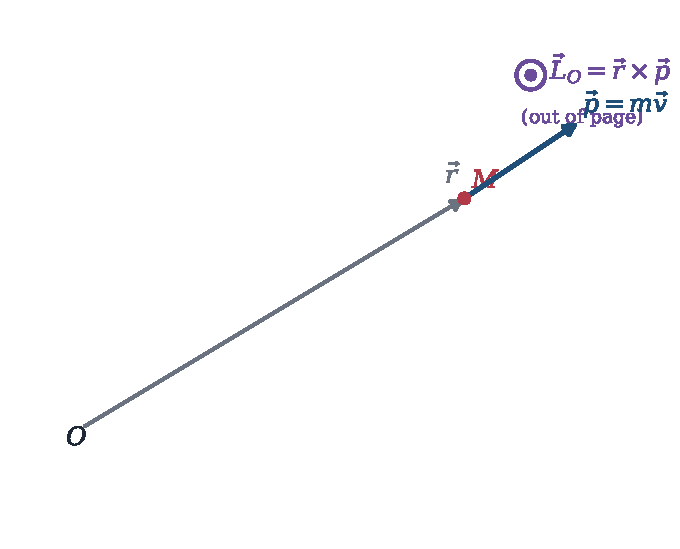
\includegraphics[width=0.72\textwidth]{figures/22_angular_momentum.pdf}
\caption{The position vector $\vec{r}$, linear momentum $\vec{p} = m\vec{v}$, and angular momentum vector $\vec{L}_O = \vec{r}\times\vec{p}$ perpendicular to the plane of motion.}
\label{fig:angular_momentum}
\end{figure}

\section{Central Forces and Conservation of Angular Momentum}

A force is called a \textbf{central force} with center $O$ if it is always directed along the line joining $O$ to the particle:
\[
\vec{F}(\vec{r}) = F(r)\,\ur, \quad \text{where } \ur = \frac{\vec{r}}{r}.
\]

\begin{keyidea}[Key Properties of Motion under a Central Force]
\begin{enumerate}[leftmargin=1.5em,itemsep=2pt]
  \item \textbf{Torque is identically zero}: $\vec{\tau}_O = \vec{r}\times(F(r)\ur) = \vzero$.
  \item \textbf{Angular momentum is strictly conserved}:
        \[
        \frac{\dd\vec{L}_O}{\dd t} = \vzero \implies \vec{L}_O = \vec{L}_0 = \text{constant vector}.
        \]
  \item \textbf{Planar trajectory}: Since $\vec{r}\cdot\vec{L}_0 = \vec{r}\cdot(\vec{r}\times\vec{p}) = 0$, the particle remains forever in the fixed plane passing through $O$ orthogonal to $\vec{L}_0$.
  \item \textbf{Constant areal velocity (Kepler's Second Law)}: In polar coordinates $(r, \theta)$ in the orbital plane:
        \[
        \vec{L}_O = m r\ur\times(\dot{r}\ur + r\dot{\theta}\ut) = m r^2\dot{\theta}\,\khat \implies \boxed{r^2\dot{\theta} = C = \frac{L_z}{m} = \text{constant},}
        \]
        where $C$ is the \emph{areal constant}. The rate at which area is swept out by the radius vector is:
        \[
        \frac{\dd A}{\dd t} = \frac{1}{2}r^2\dot{\theta} = \frac{C}{2} = \text{constant}.
        \]
\end{enumerate}
\end{keyidea}

\begin{figure}[htbp]
\centering
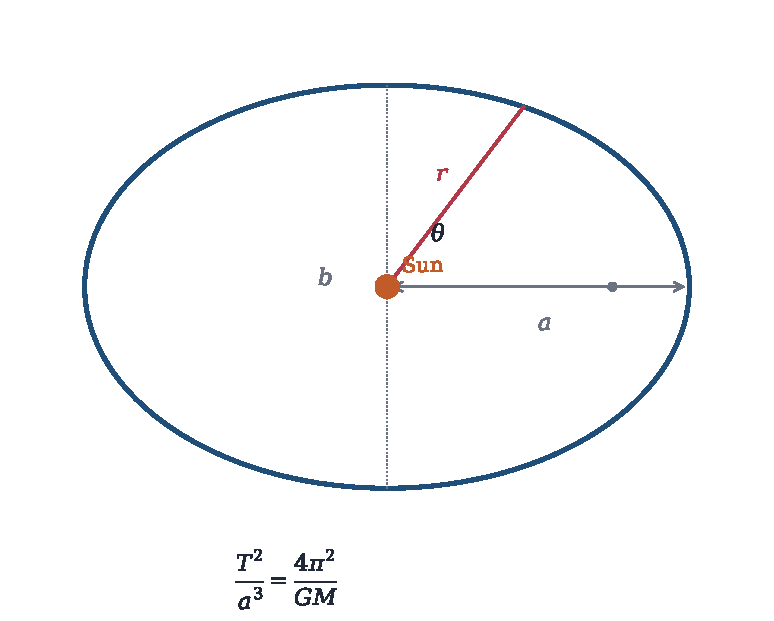
\includegraphics[width=0.74\textwidth]{figures/17_kepler.pdf}
\caption{An elliptical Keplerian orbit with the central body at one focus. Equal areas are swept out in equal times ($\Delta t_1 = \Delta t_2 \implies \Delta A_1 = \Delta A_2$).}
\label{fig:kepler_orbit}
\end{figure}

\section{The Effective Potential}

Since every central force $\vec{F} = F(r)\ur$ is conservative ($\vec{\nabla}\times\vec{F} = \vzero$), it possesses a potential energy $U(r)$ such that $F(r) = -\frac{\dd U}{\dd r}$.
The total mechanical energy in polar coordinates is:
\[
E_m = \frac{1}{2}m\left(\dot{r}^2 + r^2\dot{\theta}^2\right) + U(r).
\]
Substituting $r\dot{\theta} = \frac{L}{mr}$ reduces the 2D problem to an equivalent \textbf{one-dimensional radial motion}:
\[
\boxed{E_m = \frac{1}{2}m\dot{r}^2 + U_{\text{eff}}(r)}
\]
where the \textbf{effective potential} is:
\[
\boxed{U_{\text{eff}}(r) = U(r) + \frac{L^2}{2mr^2}.}
\]
The extra term $\frac{L^2}{2mr^2}$ is the \textbf{centrifugal barrier}, which prevents a particle with non-zero angular momentum from falling into the origin.

\section{Worked Examples}

\begin{worked}[Angular momentum of a projectile]
A projectile of mass $m$ is launched from the origin with initial velocity $\vec{v}_0 = v_0\cos\alpha\,\ihat + v_0\sin\alpha\,\jhat$ under gravity $\vec{g} = -g\jhat$.
(a) Find the angular momentum $\vec{L}_O(t)$ about the launch point $O$.
(b) Verify that $\frac{\dd\vec{L}_O}{\dd t} = \vec{\tau}_O(t)$.
\end{worked}

\begin{solution}{11.1}
(a) The position and velocity as functions of time are:
\[
\vec{r}(t) = (v_0\cos\alpha\,t)\ihat + \left(v_0\sin\alpha\,t - \frac{1}{2}gt^2\right)\jhat,
\]
\[
\vec{v}(t) = (v_0\cos\alpha)\ihat + (v_0\sin\alpha - gt)\jhat.
\]
The angular momentum about $O$ is:
\begin{align*}
\vec{L}_O(t) &= m\,\vec{r}\times\vec{v} = m\left[ x v_y - y v_x \right]\khat \\
&= m\left[ (v_0\cos\alpha\,t)(v_0\sin\alpha - gt) - \left(v_0\sin\alpha\,t - \frac{1}{2}gt^2\right)(v_0\cos\alpha) \right]\khat \\
&= m\left[ v_0^2\sin\alpha\cos\alpha\,t - g v_0\cos\alpha\,t^2 - v_0^2\sin\alpha\cos\alpha\,t + \frac{1}{2}g v_0\cos\alpha\,t^2 \right]\khat \\
&= \boxed{-\frac{1}{2}m g v_0\cos\alpha\,t^2\,\khat.}
\end{align*}

(b) The torque about $O$ due to gravity $\vec{P} = -mg\jhat$ is:
\[
\vec{\tau}_O = \vec{r}\times(-mg\jhat) = (x\ihat + y\jhat)\times(-mg\jhat) = -mgx\,\khat = -mg(v_0\cos\alpha\,t)\,\khat.
\]
Differentiating $\vec{L}_O(t)$:
\[
\frac{\dd\vec{L}_O}{\dd t} = \frac{\dd}{\dd t}\left(-\frac{1}{2}mgv_0\cos\alpha\,t^2\,\khat\right) = -mgv_0\cos\alpha\,t\,\khat = \vec{\tau}_O.
\]
The angular momentum theorem is verified!
\end{solution}

\begin{worked}[Perihelion and aphelion velocities in an elliptical orbit]
A satellite of mass $m$ orbits Earth (mass $M_E$) in an elliptical orbit. Its closest approach (perigee) is at distance $r_p$ and its farthest distance (apogee) is $r_a$. Express the speeds $v_p$ and $v_a$ in terms of $G, M_E, r_p, r_a$.
\end{worked}

\begin{solution}{11.2}
At both perigee and apogee, the velocity vector is perpendicular to the position vector ($\dot{r} = 0$).
\begin{itemize}[leftmargin=1.4em,itemsep=2pt]
  \item By conservation of angular momentum:
        \[
        L = m r_p v_p = m r_a v_a \implies v_a = \frac{r_p}{r_a}v_p.
        \]
  \item By conservation of mechanical energy:
        \[
        E_m = \frac{1}{2}mv_p^2 - \frac{GM_E m}{r_p} = \frac{1}{2}mv_a^2 - \frac{GM_E m}{r_a}.
        \]
\end{itemize}
Substituting $v_a = \frac{r_p}{r_a}v_p$:
\[
\frac{1}{2}v_p^2\left(1 - \frac{r_p^2}{r_a^2}\right) = GM_E\left(\frac{1}{r_p} - \frac{1}{r_a}\right) = GM_E\frac{r_a - r_p}{r_p r_a}.
\]
Notice that $1 - \frac{r_p^2}{r_a^2} = \frac{r_a^2 - r_p^2}{r_a^2} = \frac{(r_a - r_p)(r_a + r_p)}{r_a^2}$.
Cancelling the factor $(r_a - r_p)$:
\[
\frac{1}{2}v_p^2\frac{r_a + r_p}{r_a^2} = \frac{GM_E}{r_p r_a} \implies \boxed{v_p = \sqrt{\frac{2GM_E\,r_a}{r_p(r_p + r_a)}}.}
\]
By symmetry:
\[
\boxed{v_a = \sqrt{\frac{2GM_E\,r_p}{r_a(r_p + r_a)}}.}
\]
Since the semi-major axis is $a = \frac{r_p + r_a}{2}$, this can also be written in the famous \emph{vis-viva} form: $v^2 = GM_E\left(\frac{2}{r} - \frac{1}{a}\right)$.
\end{solution}

\section{Exercises and Step-by-Step Solutions}

\begin{exercise}{\warm\ Angular momentum in uniform rectilinear motion}
A particle of mass $m=0.50\ \mathrm{kg}$ travels at constant velocity $\vec{v} = 12.0\,\ihat\ \mathrm{m\,s^{-1}}$ along the line $y = 3.00\ \mathrm{m}$.
(a) Compute its angular momentum $\vec{L}_O$ about the origin $O(0,0)$ as a function of its $x$-coordinate.
(b) Does $\vec{L}_O$ depend on time or position? Explain why using the concept of torque.
\end{exercise}

\begin{tabletworkspace}[5.0cm]
\end{tabletworkspace}

\begin{solution}{11.1}
(a) The position vector is $\vec{r}(t) = x(t)\ihat + y_0\jhat$ with $y_0 = 3.00\ \mathrm{m}$.
The velocity is $\vec{v} = v_0\ihat$ with $v_0 = 12.0\ \mathrm{m\,s^{-1}}$.
The angular momentum about $O$ is:
\[
\vec{L}_O = \vec{r}\times(m\vec{v}) = (x\ihat + y_0\jhat)\times(m v_0\ihat) = -m v_0 y_0\,\khat.
\]
Substituting the numerical values:
\[
\vec{L}_O = -(0.50)(12.0)(3.00)\,\khat = \mathbf{-18.0\,\khat\ \mathrm{kg\,m^2\,s^{-1}}.}
\]

(b) $\vec{L}_O$ is strictly constant: it is completely independent of $x$ and $t$.
This is because the particle is in uniform rectilinear motion ($\vec{a} = \vzero$), so the net force is zero ($\vec{F} = \vzero$), meaning the net torque about the origin is $\vec{\tau}_O = \vec{r}\times\vec{F} = \vzero$. By the angular momentum theorem, $\frac{\dd\vec{L}_O}{\dd t} = \vzero$, so $\vec{L}_O = \text{const}$. Geometrically, $\norm{\vec{L}_O} = m v_0 d$, where $d = y_0$ is the perpendicular distance (impact parameter) from $O$ to the line of motion.
\end{solution}

\begin{exercise}{\warm\ Circular orbit speed and period of the ISS}
The International Space Station (ISS) orbits Earth in an approximately circular orbit at an altitude of $h = 415\ \mathrm{km}$ above Earth's surface.
(Earth's radius $R_E = 6371\ \mathrm{km}$, Earth's mass $M_E = 5.972\times 10^{24}\ \mathrm{kg}$, $G = 6.674\times 10^{-11}\ \mathrm{m^3\,kg^{-1}\,s^{-2}}$).
(a) Using Newton's second law, find the orbital speed $v_c$.
(b) Compute the orbital period $T$ in minutes.
(c) How many revolutions does the ISS complete in 24 hours?
\end{exercise}

\begin{tabletworkspace}[5.5cm]
\end{tabletworkspace}

\begin{solution}{11.2}
(a) The orbital radius is $r = R_E + h = 6371 + 415 = 6786\ \mathrm{km} = 6.786\times 10^6\ \mathrm{m}$.
For circular motion under gravity:
\[
m\frac{v_c^2}{r} = \frac{GM_E m}{r^2} \implies \boxed{v_c = \sqrt{\frac{GM_E}{r}}.}
\]
Computing:
\[
v_c = \sqrt{\frac{(6.674\times 10^{-11})(5.972\times 10^{24})}{6.786\times 10^6}} = \sqrt{\frac{3.986\times 10^{14}}{6.786\times 10^6}} = \sqrt{5.874\times 10^7} \approx 7664\ \mathrm{m\,s^{-1}} \approx \mathbf{7.66\ \mathrm{km\,s^{-1}}.}
\]

(b) The orbital period is:
\[
T = \frac{2\pi r}{v_c} = \frac{2\pi(6.786\times 10^6)}{7664} \approx 5563\ \mathrm{s} \approx \mathbf{92.7\ \mathrm{min}} \quad (1\ \mathrm{h}\ 32.7\ \mathrm{min}).
\]

(c) Number of orbits per day (24 hours = 1440 min):
\[
N = \frac{1440}{92.72} \approx \mathbf{15.5\ \text{orbits per day}}.
\]
\end{solution}

\begin{exercise}{\warm\ Escape velocity from celestial bodies}
The escape velocity $v_{\text{esc}}$ is the minimum speed needed for a projectile launched from the surface of a body to escape its gravitational pull completely ($r \to \infty$).
(a) Using conservation of mechanical energy, show that $v_{\text{esc}} = \sqrt{\frac{2GM}{R}} = \sqrt{2gR}$.
(b) Calculate $v_{\text{esc}}$ for Earth ($R_E = 6371\ \mathrm{km}, g = 9.81\ \mathrm{m\,s^{-2}}$).
(c) Calculate $v_{\text{esc}}$ for the Moon ($M_M = 7.342\times 10^{22}\ \mathrm{kg}, R_M = 1737\ \mathrm{km}$).
\end{exercise}

\begin{tabletworkspace}[5.0cm]
\end{tabletworkspace}

\begin{solution}{11.3}
(a) Mechanical energy at launch ($r = R$, $v = v_{\text{esc}}$):
\[
E_m = \frac{1}{2}m v_{\text{esc}}^2 - \frac{GMm}{R}.
\]
At infinity ($r \to \infty$), the gravitational potential energy vanishes ($U \to 0$), and the condition for just escaping is that the speed reaches zero ($v \ge 0$), so $E_{m, \infty} \ge 0$.
By conservation of energy:
\[
\frac{1}{2}m v_{\text{esc}}^2 - \frac{GMm}{R} = 0 \implies \boxed{v_{\text{esc}} = \sqrt{\frac{2GM}{R}}.}
\]
Since $g = \frac{GM}{R^2}$, we have $\frac{GM}{R} = gR$, so $v_{\text{esc}} = \sqrt{2gR}$.

(b) For Earth:
\[
v_{\text{esc}, E} = \sqrt{2(9.81)(6.371\times 10^6)} = \sqrt{1.250\times 10^8} \approx 11180\ \mathrm{m\,s^{-1}} = \mathbf{11.2\ \mathrm{km\,s^{-1}}.}
\]

(c) For the Moon:
\[
v_{\text{esc}, M} = \sqrt{\frac{2(6.674\times 10^{-11})(7.342\times 10^{22})}{1.737\times 10^6}} = \sqrt{\frac{9.800\times 10^{12}}{1.737\times 10^6}} = \sqrt{5.642\times 10^6} \approx 2375\ \mathrm{m\,s^{-1}} = \mathbf{2.38\ \mathrm{km\,s^{-1}}.}
\]
The Moon's escape velocity is nearly 5 times smaller than Earth's, which explains why the Moon could not retain an atmosphere.
\end{solution}

\begin{exercise}{\core\ Mass on a table with a hole: pulling the string}
A small puck of mass $m=0.20\ \mathrm{kg}$ on a frictionless horizontal table is connected to a light string passing through a small hole at the center $O$. The puck initially moves in a circle of radius $r_1 = 0.50\ \mathrm{m}$ with speed $v_1 = 2.0\ \mathrm{m\,s^{-1}}$. The string is then slowly pulled from below until the radius of the circular path is reduced to $r_2 = 0.25\ \mathrm{m}$.
(a) Explain why angular momentum about $O$ is conserved during the process.
(b) Find the new speed $v_2$ of the puck.
(c) Find the initial and final tension in the string.
(d) Calculate the work done by the person pulling the string using the work-energy theorem.
\end{exercise}

\begin{tabletworkspace}[6.0cm]
\end{tabletworkspace}

\begin{solution}{11.4}
(a) The string tension $\vec{T} = -T\ur$ is always directed toward the central hole $O$. The torque about $O$ is:
\[
\vec{\tau}_O = \vec{r}\times\vec{T} = r\ur\times(-T\ur) = \vzero.
\]
Therefore, angular momentum about $O$ is strictly conserved: $L = m r_1 v_1 = m r_2 v_2 = \text{const}$.

(b) Conserving angular momentum:
\[
v_2 = \frac{r_1}{r_2} v_1 = \frac{0.50}{0.25}\times 2.0 = 2\times 2.0 = \mathbf{4.0\ \mathrm{m\,s^{-1}}.}
\]

(c) The tension provides the centripetal acceleration $T = \frac{m v^2}{r}$:
\begin{align*}
T_1 &= \frac{m v_1^2}{r_1} = \frac{0.20\times (2.0)^2}{0.50} = \frac{0.80}{0.50} = \mathbf{1.60\ \mathrm{N},} \\
T_2 &= \frac{m v_2^2}{r_2} = \frac{0.20\times (4.0)^2}{0.25} = \frac{3.20}{0.25} = \mathbf{12.8\ \mathrm{N}.}
\end{align*}
The tension increases by a factor of $(r_1/r_2)^3 = 2^3 = 8$!

(d) By the work-energy theorem, since the normal force and gravity cancel and do no work, the work done by the tension force is the change in kinetic energy:
\[
W = \Delta E_c = \frac{1}{2}m v_2^2 - \frac{1}{2}m v_1^2 = \frac{1}{2}(0.20)\left[ 4.0^2 - 2.0^2 \right] = 0.10(16 - 4) = 0.10\times 12 = \mathbf{1.20\ \mathrm{J}.}
\]
The person pulling the string performs $+1.20\ \mathrm{J}$ of positive work against the centrifugal effect.
\end{solution}

\begin{exercise}{\core\ Effective potential and turning points}
A particle of mass $m$ moves under an attractive central force with potential $U(r) = -\frac{k}{r}$ ($k > 0$). Its angular momentum is $L$.
(a) Write down the effective potential $U_{\text{eff}}(r)$ and sketch it as a function of $r$.
(b) Find the radius $r_0$ of the circular orbit where $U_{\text{eff}}$ has its minimum, and compute the minimum energy $E_{\min} = U_{\text{eff}}(r_0)$.
(c) For total energy $E_m$ such that $E_{\min} < E_m < 0$, find the turning points $r_{\min}$ (periapsis) and $r_{\max}$ (apoapsis) in terms of $E_m, L, m, k$.
\end{exercise}

\begin{tabletworkspace}[6.5cm]
\end{tabletworkspace}

\begin{solution}{11.5}
(a) The effective potential is:
\[
\boxed{U_{\text{eff}}(r) = -\frac{k}{r} + \frac{L^2}{2mr^2}.}
\]
As $r \to 0$, the centrifugal term $\frac{L^2}{2mr^2} \to +\infty$ dominates (repulsive barrier).
As $r \to \infty$, $U_{\text{eff}}(r) \to 0^-$ (governed by $-\frac{k}{r}$).
In between, it exhibits a unique negative potential well minimum.

(b) The minimum occurs where $\frac{\dd U_{\text{eff}}}{\dd r} = 0$:
\[
\frac{\dd U_{\text{eff}}}{\dd r} = \frac{k}{r^2} - \frac{L^2}{mr^3} = 0 \implies \frac{k}{r_0^2} = \frac{L^2}{mr_0^3} \implies \boxed{r_0 = \frac{L^2}{mk}.}
\]
The second derivative is:
\[
\frac{\dd^2 U_{\text{eff}}}{\dd r^2} = -\frac{2k}{r^3} + \frac{3L^2}{mr^4} \implies \left.\frac{\dd^2 U_{\text{eff}}}{\dd r^2}\right|_{r_0} = -\frac{2k}{(L^2/mk)^3} + \frac{3L^2}{m(L^2/mk)^4} = \frac{m^3 k^4}{L^6} > 0,
\]
confirming a stable circular orbit!
The minimum energy is:
\[
E_{\min} = U_{\text{eff}}(r_0) = -\frac{k}{L^2/(mk)} + \frac{L^2}{2m(L^2/mk)^2} = -\frac{mk^2}{L^2} + \frac{mk^2}{2L^2} = \boxed{-\frac{mk^2}{2L^2}.}
\]

(c) Turning points are where the radial velocity vanishes: $\dot{r} = 0 \iff E_m = U_{\text{eff}}(r)$:
\[
E_m = -\frac{k}{r} + \frac{L^2}{2mr^2} \iff E_m r^2 + kr - \frac{L^2}{2m} = 0.
\]
Dividing by $E_m$ (with $E_m < 0$, let $\abs{E_m} = -E_m$):
\[
r^2 - \frac{k}{\abs{E_m}}r + \frac{L^2}{2m\abs{E_m}} = 0.
\]
Solving the quadratic equation:
\[
\Delta = \frac{k^2}{E_m^2} - \frac{2L^2}{m\abs{E_m}} = \frac{k^2}{E_m^2}\left(1 - \frac{2\abs{E_m}L^2}{mk^2}\right) = \frac{k^2}{E_m^2}\left(1 - \frac{\abs{E_m}}{\abs{E_{\min}}}\right).
\]
Since $E_{\min} < E_m < 0$, $\Delta > 0$. The two roots are:
\[
\boxed{r_{\min, \max} = \frac{k}{2\abs{E_m}}\left[ 1 \mp \sqrt{1 - \frac{2\abs{E_m}L^2}{mk^2}} \right].}
\]
Notice that the semi-major axis is $a = \frac{r_{\min} + r_{\max}}{2} = \frac{k}{2\abs{E_m}} \implies E_m = -\frac{k}{2a}$, and the eccentricity is $e = \sqrt{1 - \frac{2\abs{E_m}L^2}{mk^2}}$.
\end{solution}

\begin{exercise}{\core\ Hohmann Transfer Orbit to Mars}
A spacecraft is in a circular parking orbit around the Sun at Earth's distance $r_1 = 1.00\ \mathrm{AU} = 1.496\times 10^{11}\ \mathrm{m}$. It needs to transfer to Mars's orbit, assumed circular at $r_2 = 1.524\ \mathrm{AU} = 2.280\times 10^{11}\ \mathrm{m}$.
The Sun's gravitational parameter is $\mu = GM_\odot = 1.327\times 10^{20}\ \mathrm{m^3\,s^{-2}}$.
(a) Find the semi-major axis $a_{\text{trans}}$ of the elliptical Hohmann transfer orbit.
(b) Calculate the travel time (in days) to reach Mars.
(c) Compute the initial velocity increment $\Delta v_1$ required to leave Earth's orbit and enter the transfer ellipse.
\end{exercise}

\begin{tabletworkspace}[6.5cm]
\end{tabletworkspace}

\begin{solution}{11.6}
(a) The Hohmann transfer orbit is an ellipse with perihelion at Earth's orbit ($r_p = r_1$) and aphelion at Mars's orbit ($r_a = r_2$).
The major axis is $2a_{\text{trans}} = r_1 + r_2$, so:
\[
a_{\text{trans}} = \frac{r_1 + r_2}{2} = \frac{1.000 + 1.524}{2} = \mathbf{1.262\ \mathrm{AU}} = 1.262\times(1.496\times 10^{11}) = \mathbf{1.888\times 10^{11}\ \mathrm{m}.}
\]

(b) By Kepler's third law, the period of the complete ellipse is:
\[
T_{\text{trans}} = T_{\text{Earth}} \left(\frac{a_{\text{trans}}}{a_1}\right)^{3/2} = 1.00\ \text{year}\times(1.262)^{3/2} = 1.00\times 1.418 = 1.418\ \text{years}.
\]
The flight time to Mars is half of this orbital period (from perihelion to aphelion):
\[
t_{\text{flight}} = \frac{1}{2}T_{\text{trans}} = \frac{1.418\times 365.25}{2} \approx \mathbf{259\ \text{days}} \quad (\approx 8.5\ \text{months}).
\]

(c) Earth's circular orbital speed:
\[
v_{c1} = \sqrt{\frac{\mu}{r_1}} = \sqrt{\frac{1.327\times 10^{20}}{1.496\times 10^{11}}} \approx 29780\ \mathrm{m\,s^{-1}} = 29.78\ \mathrm{km\,s^{-1}}.
\]
The required perihelion speed on the transfer ellipse (using the \emph{vis-viva} equation $v^2 = \mu\left(\frac{2}{r} - \frac{1}{a}\right)$):
\[
v_{p} = \sqrt{\mu\left(\frac{2}{r_1} - \frac{1}{a_{\text{trans}}}\right)} = \sqrt{(1.327\times 10^{20})\left(\frac{2}{1.496\times 10^{11}} - \frac{1}{1.888\times 10^{11}}\right)} \approx 32730\ \mathrm{m\,s^{-1}} = 32.73\ \mathrm{km\,s^{-1}}.
\]
The required impulse at departure is:
\[
\Delta v_1 = v_p - v_{c1} = 32.73 - 29.78 = \mathbf{2.95\ \mathrm{km\,s^{-1}}.}
\]
\end{solution}

\begin{exercise}{\mastery\ Binet's Formulas and Kepler's First Law}
In polar coordinates $(r, \theta)$, define $u(\theta) = \frac{1}{r(\theta)}$.
(a) Using $r^2\dot{\theta} = C$, show that:
\[
\dot{r} = -C\frac{\dd u}{\dd\theta},\qquad \ddot{r} - r\dot{\theta}^2 = -C^2 u^2\left(\frac{\dd^2 u}{\dd\theta^2} + u\right).
\]
(b) Deduce \textbf{Binet's formula for acceleration}:
\[
a_r = -C^2 u^2\left(\frac{\dd^2 u}{\dd\theta^2} + u\right).
\]
(c) An observed orbit is an ellipse with the force center at one focus: $r(\theta) = \frac{p}{1 + e\cos\theta}$. Prove that the central force must be an inverse-square law $F(r) \propto -\frac{1}{r^2}$.
\end{exercise}

\begin{tabletworkspace}[6.5cm]
\end{tabletworkspace}

\begin{solution}{11.7}
(a) Using the chain rule $\frac{\dd}{\dd t} = \dot{\theta}\frac{\dd}{\dd\theta} = \frac{C}{r^2}\frac{\dd}{\dd\theta} = Cu^2\frac{\dd}{\dd\theta}$:
\[
\dot{r} = \frac{\dd}{\dd t}\left(\frac{1}{u}\right) = -\frac{1}{u^2}\dot{u} = -\frac{1}{u^2}\left(Cu^2\frac{\dd u}{\dd\theta}\right) = \boxed{-C\frac{\dd u}{\dd\theta}.}
\]
Differentiating again with respect to $t$:
\[
\ddot{r} = \frac{\dd}{\dd t}\left(-C\frac{\dd u}{\dd\theta}\right) = Cu^2\frac{\dd}{\dd\theta}\left(-C\frac{\dd u}{\dd\theta}\right) = -C^2 u^2\frac{\dd^2 u}{\dd\theta^2}.
\]
The second centripetal term is:
\[
r\dot{\theta}^2 = \frac{1}{u}\left(Cu^2\right)^2 = C^2 u^3.
\]
Combining the terms:
\[
\ddot{r} - r\dot{\theta}^2 = -C^2 u^2\frac{\dd^2 u}{\dd\theta^2} - C^2 u^3 = \boxed{-C^2 u^2\left(\frac{\dd^2 u}{\dd\theta^2} + u\right).}
\]

(b) In polar coordinates, the radial acceleration is precisely $a_r = \ddot{r} - r\dot{\theta}^2$. Therefore:
\[
\boxed{a_r = -C^2 u^2\left(\frac{\dd^2 u}{\dd\theta^2} + u\right).}
\]
Newton's second law $m a_r = F(r)$ gives Binet's equation:
\[
F(1/u) = -m C^2 u^2\left(\frac{\dd^2 u}{\dd\theta^2} + u\right).
\]

(c) Given the focal ellipse equation $r(\theta) = \frac{p}{1 + e\cos\theta}$:
\[
u(\theta) = \frac{1}{r(\theta)} = \frac{1}{p} + \frac{e}{p}\cos\theta.
\]
Differentiating twice with respect to $\theta$:
\[
\frac{\dd u}{\dd\theta} = -\frac{e}{p}\sin\theta,\qquad \frac{\dd^2 u}{\dd\theta^2} = -\frac{e}{p}\cos\theta.
\]
Adding $u$:
\[
\frac{\dd^2 u}{\dd\theta^2} + u = -\frac{e}{p}\cos\theta + \left(\frac{1}{p} + \frac{e}{p}\cos\theta\right) = \frac{1}{p} = \text{constant!}
\]
Substituting into Binet's force formula:
\[
F(r) = -m C^2 u^2\left(\frac{1}{p}\right) = -\frac{m C^2}{p} u^2 = \boxed{-\frac{m C^2}{p}\frac{1}{r^2}.}
\]
This completes Newton's celebrated deduction: an elliptical orbit with the focus at the center of force uniquely requires an \textbf{inverse-square gravitational force} $F(r) \propto -\frac{1}{r^2}$!
\end{solution}

\begin{exercise}{\mastery\ Rutherford Scattering: Repulsive Central Force}
An alpha particle of mass $m$ and charge $q_1 = +2e$ is fired with initial speed $v_0$ and impact parameter $b$ toward a stationary heavy gold nucleus of charge $q_2 = +Ze$.
The Coulomb repulsive force is $\vec{F} = \frac{k}{r^2}\ur$, where $k = \frac{q_1 q_2}{4\pi\varepsilon_0}$.
(a) Write the conservation of angular momentum $L$ and total mechanical energy $E_m$ in terms of $m, v_0, b$.
(b) Using Binet's equation $\frac{\dd^2 u}{\dd\theta^2} + u = -\frac{m k}{L^2}$, show that the trajectory is a hyperbola:
\[
u(\theta) = \frac{1}{r(\theta)} = \frac{1}{p}\left(e\cos\theta - 1\right),
\]
where $p = \frac{L^2}{mk}$.
(c) Deduce Rutherford's scattering formula relating the deflection angle $\theta_s$ to the impact parameter $b$:
\[
\tan\left(\frac{\theta_s}{2}\right) = \frac{k}{m v_0^2 b}.
\]
\end{exercise}

\begin{tabletworkspace}[6.5cm]
\end{tabletworkspace}

\begin{solution}{11.8}
(a) At $r \to \infty$, the particle moves with speed $v_0$ along a line at distance $b$ from the nucleus:
\[
L = m v_0 b = \text{const},\qquad E_m = \frac{1}{2}m v_0^2 = \text{const}.
\]

(b) Binet's equation for a repulsive force $F(r) = +\frac{k}{r^2} = +k u^2$:
\[
-m C^2 u^2\left(\frac{\dd^2 u}{\dd\theta^2} + u\right) = k u^2 \implies \frac{\dd^2 u}{\dd\theta^2} + u = -\frac{k}{m C^2} = -\frac{mk}{L^2}.
\]
Defining $p = \frac{L^2}{mk}$, this is a harmonic oscillator with constant drive:
\[
\frac{\dd^2 u}{\dd\theta^2} + u = -\frac{1}{p}.
\]
The general solution is:
\[
u(\theta) = A\cos(\theta - \theta_0) - \frac{1}{p}.
\]
Aligning the symmetry axis (periapsis at $\theta = 0$):
\[
u(\theta) = \frac{1}{p}\left(e\cos\theta - 1\right).
\]
Since $r > 0$, this represents the repulsive branch of a hyperbola ($e > 1$).

(c) The asymptotes of the hyperbola correspond to $r \to \infty \implies u(\theta_\infty) = 0$:
\[
e\cos\theta_\infty - 1 = 0 \implies \cos\theta_\infty = \frac{1}{e}.
\]
From the geometry of hyperbolic scattering, the incoming direction is $-\theta_\infty$ and the outgoing direction is $+\theta_\infty$.
The total deflection (scattering angle) is $\theta_s = \pi - 2\theta_\infty \implies \theta_\infty = \frac{\pi - \theta_s}{2}$.
Thus:
\[
\cos\theta_\infty = \cos\left(\frac{\pi}{2} - \frac{\theta_s}{2}\right) = \sin\left(\frac{\theta_s}{2}\right) = \frac{1}{e}.
\]
Consequently:
\[
\cot\left(\frac{\theta_s}{2}\right) = \sqrt{e^2 - 1}.
\]
To relate $e$ to $b$, note that at periapsis $r_0 = \frac{p}{e - 1}$, and using energy conservation $E_m = \frac{k(e^2 - 1)}{2p} = \frac{1}{2}m v_0^2$:
\[
e^2 - 1 = \frac{2 E_m p}{k} = \frac{2(\frac{1}{2}m v_0^2)(m^2 v_0^2 b^2 / mk)}{k} = \left(\frac{m v_0^2 b}{k}\right)^2.
\]
Taking the square root:
\[
\cot\left(\frac{\theta_s}{2}\right) = \frac{m v_0^2 b}{k} \implies \boxed{\tan\left(\frac{\theta_s}{2}\right) = \frac{k}{m v_0^2 b}.}
\]
This is the fundamental Rutherford scattering relation that revealed the atomic nucleus in 1911!
\end{solution}

\begin{exercise}{\mastery\ Distance of Closest Approach for an Alpha Particle}
In a head-on collision ($b = 0$), an alpha particle of mass $m = 6.64\times 10^{-27}\ \mathrm{kg}$ and kinetic energy $K = 5.00\ \mathrm{MeV}$ is fired directly at a gold nucleus ($Z = 79$).
($1\ \mathrm{eV} = 1.602\times 10^{-19}\ \mathrm{J}$, $\frac{1}{4\pi\varepsilon_0} = 8.988\times 10^9\ \mathrm{N\,m^2\,C^{-2}}$, $e = 1.602\times 10^{-19}\ \mathrm{C}$).
(a) Express the distance of closest approach $d_{\min}$ using conservation of energy.
(b) Calculate $d_{\min}$ in femtometres ($\mathrm{fm} = 10^{-15}\ \mathrm{m}$).
(c) What upper bound does this place on the radius of the gold nucleus?
\end{exercise}

\begin{tabletworkspace}[5.5cm]
\end{tabletworkspace}

\begin{solution}{11.9}
(a) For a head-on collision ($b = 0$), the particle travels along a straight line. At closest approach, its speed drops momentarily to zero ($v = 0$).
By conservation of mechanical energy:
\[
E_m = K_{\infty} = U(d_{\min}) \implies K = \frac{1}{4\pi\varepsilon_0}\frac{(2e)(Ze)}{d_{\min}} = \frac{2Ze^2}{4\pi\varepsilon_0\,d_{\min}}.
\]
Solving for $d_{\min}$:
\[
\boxed{d_{\min} = \frac{2Ze^2}{4\pi\varepsilon_0 K}.}
\]

(b) Convert $K = 5.00\ \mathrm{MeV}$ to joules:
\[
K = 5.00\times 10^6\times 1.602\times 10^{-19}\ \mathrm{J} = 8.01\times 10^{-13}\ \mathrm{J}.
\]
Calculate $d_{\min}$ with $Z = 79$:
\begin{align*}
d_{\min} &= \frac{(8.988\times 10^9)\times 2\times 79\times (1.602\times 10^{-19})^2}{8.01\times 10^{-13}} \\
&= \frac{(8.988\times 10^9)\times 158\times (2.566\times 10^{-38})}{8.01\times 10^{-13}} \\
&= \frac{3.644\times 10^{-26}}{8.01\times 10^{-13}} \approx 4.55\times 10^{-14}\ \mathrm{m} = \mathbf{45.5\ \mathrm{fm}.}
\end{align*}

(c) Because the alpha particle turns around purely under electrostatic repulsion without hitting the nuclear surface, the radius of the gold nucleus must be strictly less than $d_{\min}$:
\[
R_{\text{gold}} < 45.5\ \mathrm{fm}.
\]
(The actual measured nuclear radius of gold is $R \approx 1.2 A^{1/3} \approx 1.2(197)^{1/3} \approx 7.0\ \mathrm{fm}$).
\end{solution}

\begin{exercise}{\mastery\ Precession of the Perihelion under a Perturbed Central Force}
Consider a nearly circular planetary orbit under a modified gravitational potential $U(r) = -\frac{k}{r} - \frac{\epsilon}{r^2}$, where $\epsilon$ is a tiny relativistic correction.
(a) Find the effective potential $U_{\text{eff}}(r)$ and the radius $r_0$ of the circular orbit in terms of $L, m, k, \epsilon$.
(b) Perform a Taylor expansion of $U_{\text{eff}}(r)$ around $r_0$ to second order: $U_{\text{eff}}(r) \approx U_{\text{eff}}(r_0) + \frac{1}{2}k_{\text{eff}}(r - r_0)^2$. Find the radial oscillation frequency $\omega_r = \sqrt{k_{\text{eff}}/m}$.
(c) Comparing $\omega_r$ with the orbital angular frequency $\omega_\theta = \dot{\theta} = \frac{L}{m r_0^2}$, show that the perihelion precesses by an angle $\Delta\theta_p \approx \frac{2\pi\epsilon}{k r_0}$ per orbit.
\end{exercise}

\begin{tabletworkspace}[6.5cm]
\end{tabletworkspace}

\begin{solution}{11.10}
(a) The effective potential is:
\[
U_{\text{eff}}(r) = -\frac{k}{r} - \frac{\epsilon}{r^2} + \frac{L^2}{2mr^2} = -\frac{k}{r} + \frac{L^2 - 2m\epsilon}{2mr^2}.
\]
Define the modified angular momentum parameter $L'^2 = L^2 - 2m\epsilon$.
The circular orbit occurs at the minimum:
\[
\frac{\dd U_{\text{eff}}}{\dd r} = \frac{k}{r^2} - \frac{L'^2}{mr^3} = 0 \implies \boxed{r_0 = \frac{L'^2}{mk} \approx \frac{L^2}{mk}\left(1 - \frac{2m\epsilon}{L^2}\right).}
\]

(b) Second derivative at $r_0$:
\[
\frac{\dd^2 U_{\text{eff}}}{\dd r^2} = -\frac{2k}{r^3} + \frac{3L'^2}{mr^4}.
\]
Evaluating at $r_0 = \frac{L'^2}{mk}$:
\[
k_{\text{eff}} = \left.\frac{\dd^2 U_{\text{eff}}}{\dd r^2}\right|_{r_0} = -\frac{2k}{r_0^3} + \frac{3(mkr_0)}{mr_0^4} = \frac{k}{r_0^3}.
\]
The radial oscillation frequency is:
\[
\omega_r = \sqrt{\frac{k_{\text{eff}}}{m}} = \sqrt{\frac{k}{m r_0^3}}.
\]

(c) The orbital frequency for circular motion is $\omega_\theta = \frac{L}{m r_0^2}$.
Using $\frac{L^2}{m r_0^3} = \frac{L'^2 + 2m\epsilon}{m r_0^3} = \frac{m k r_0 + 2m\epsilon}{m r_0^3} = \frac{k}{r_0^2} + \frac{2\epsilon}{r_0^3}$:
\[
\omega_\theta = \sqrt{\frac{k}{m r_0^3} + \frac{2\epsilon}{m r_0^4}} = \omega_r \sqrt{1 + \frac{2\epsilon}{k r_0}} \approx \omega_r\left(1 + \frac{\epsilon}{k r_0}\right).
\]
The time between two consecutive perihelion passages is the radial period $T_r = \frac{2\pi}{\omega_r}$.
During this time, the polar angle increases by:
\[
\Delta\theta = \omega_\theta T_r = \omega_\theta \frac{2\pi}{\omega_r} \approx 2\pi\left(1 + \frac{\epsilon}{k r_0}\right) = 2\pi + \Delta\theta_p.
\]
Therefore, the perihelion advances each orbit by:
\[
\boxed{\Delta\theta_p \approx \frac{2\pi\epsilon}{k r_0}.}
\]
This orbital precession was precisely what Einstein used in 1915 to verify General Relativity through the 43 arcseconds per century anomalous precession of Mercury's perihelion!
\end{solution}
